\documentclass{article}
\usepackage{graphicx}
\graphicspath{{images/}}

\begin{document}
\begin{itemize}
	\item For the equation $r = ((r*x)*y)*z$. \\
	\begin{figure}[h]
		\centering
		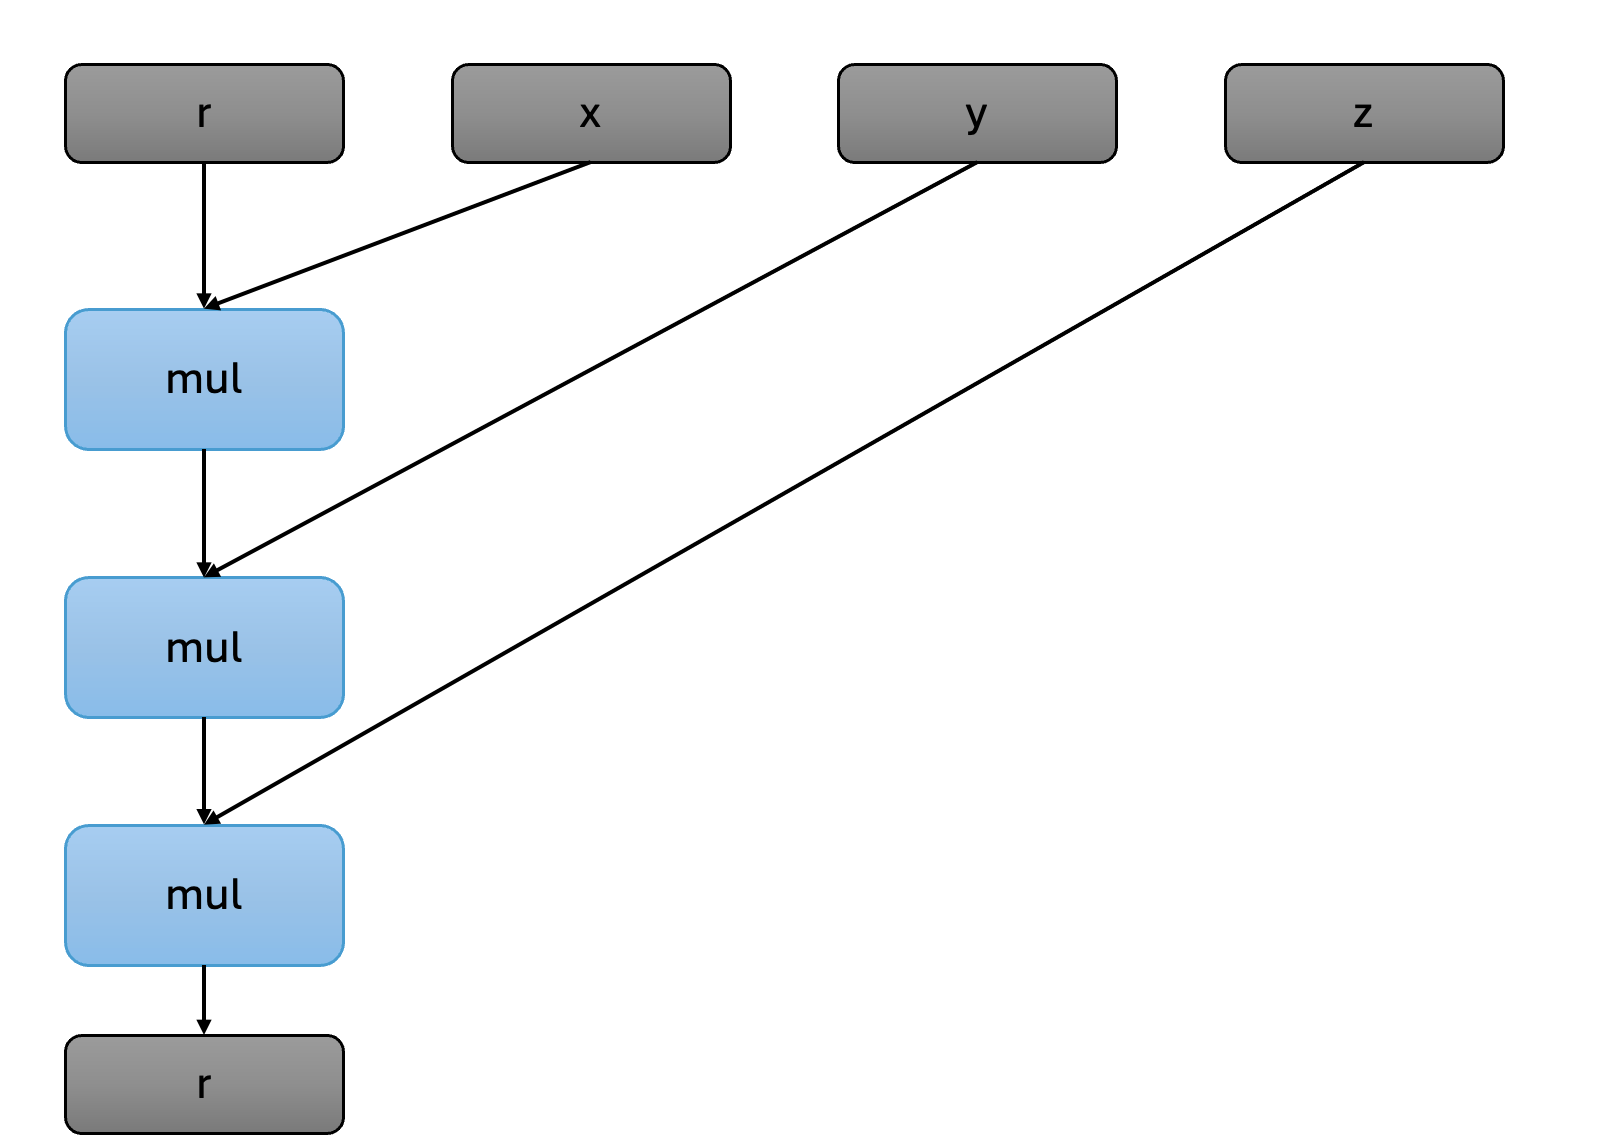
\includegraphics[width=0.5\textwidth]{fig1}
	\end{figure} \\
	The CPE is 5.0 clock cycles.
	\item For the equation $r = (r*(x*y))*z$. \\
	\begin{figure}[h]
		\centering
		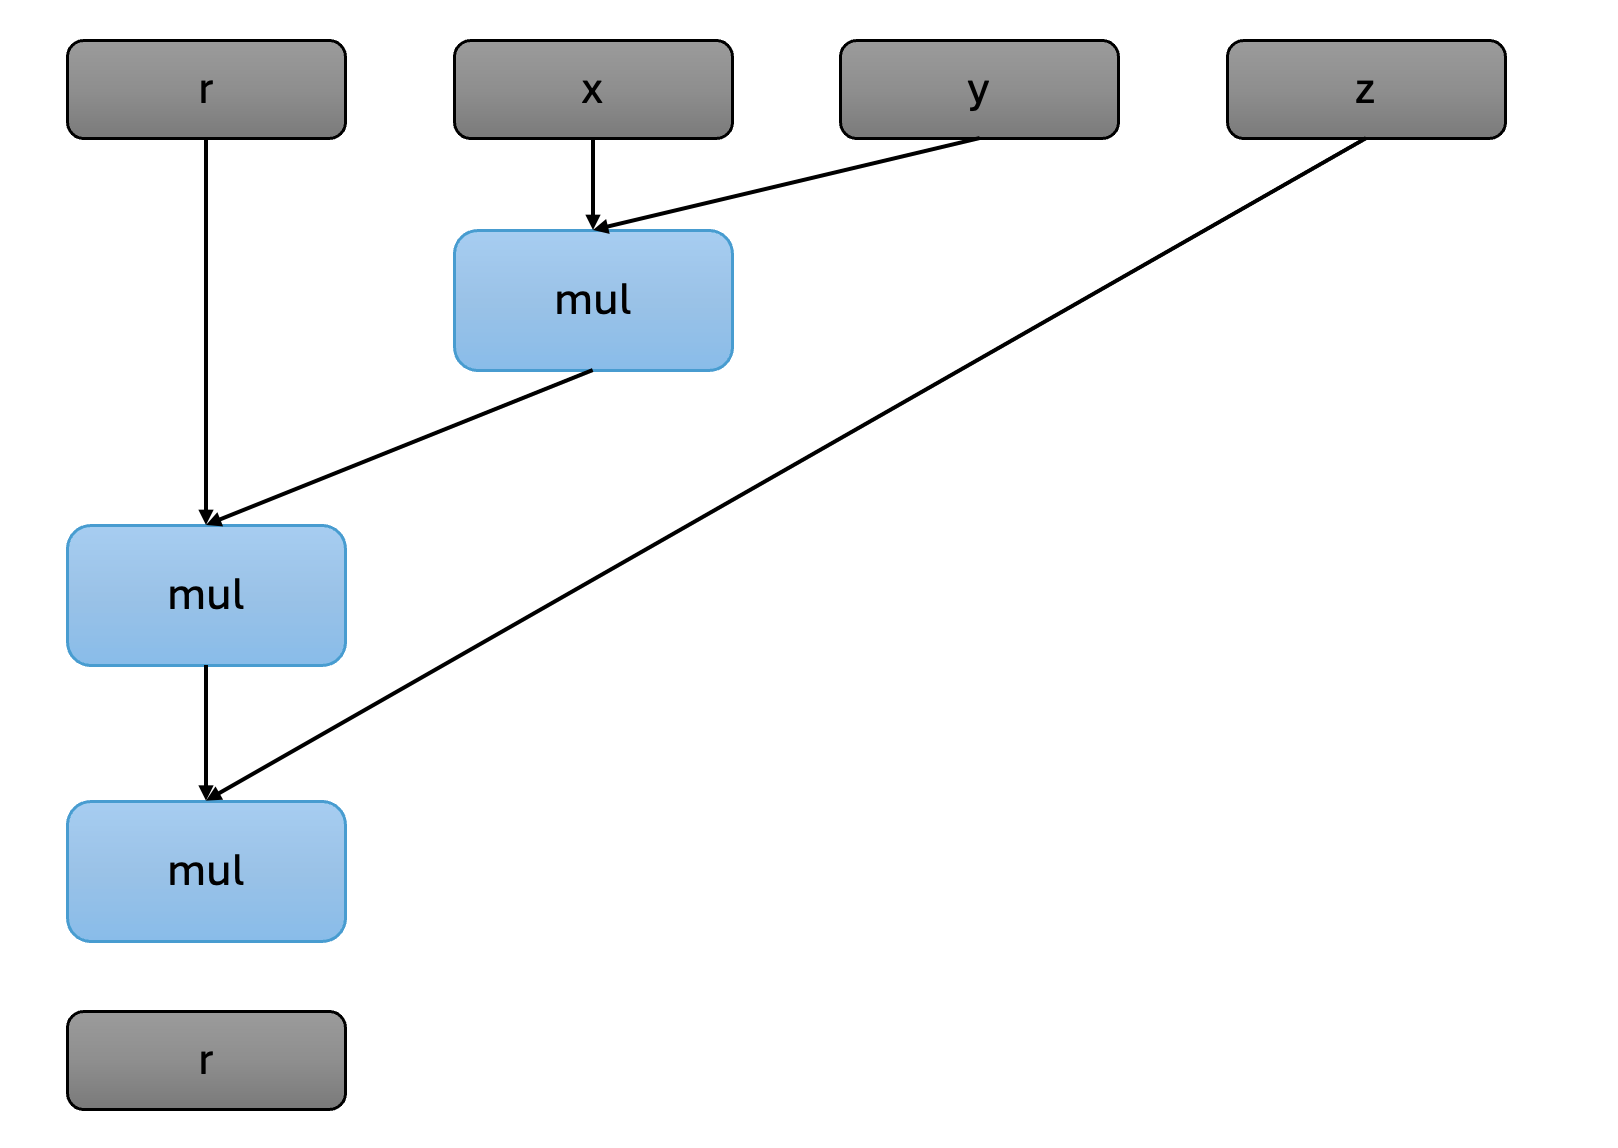
\includegraphics[width=0.5\textwidth]{fig2}
	\end{figure} \\
	The CPE is 3.33 clock cycles.
	\item For the equation $r = r*((x*y)*z)$. \\
	\begin{figure}[h]
		\centering
		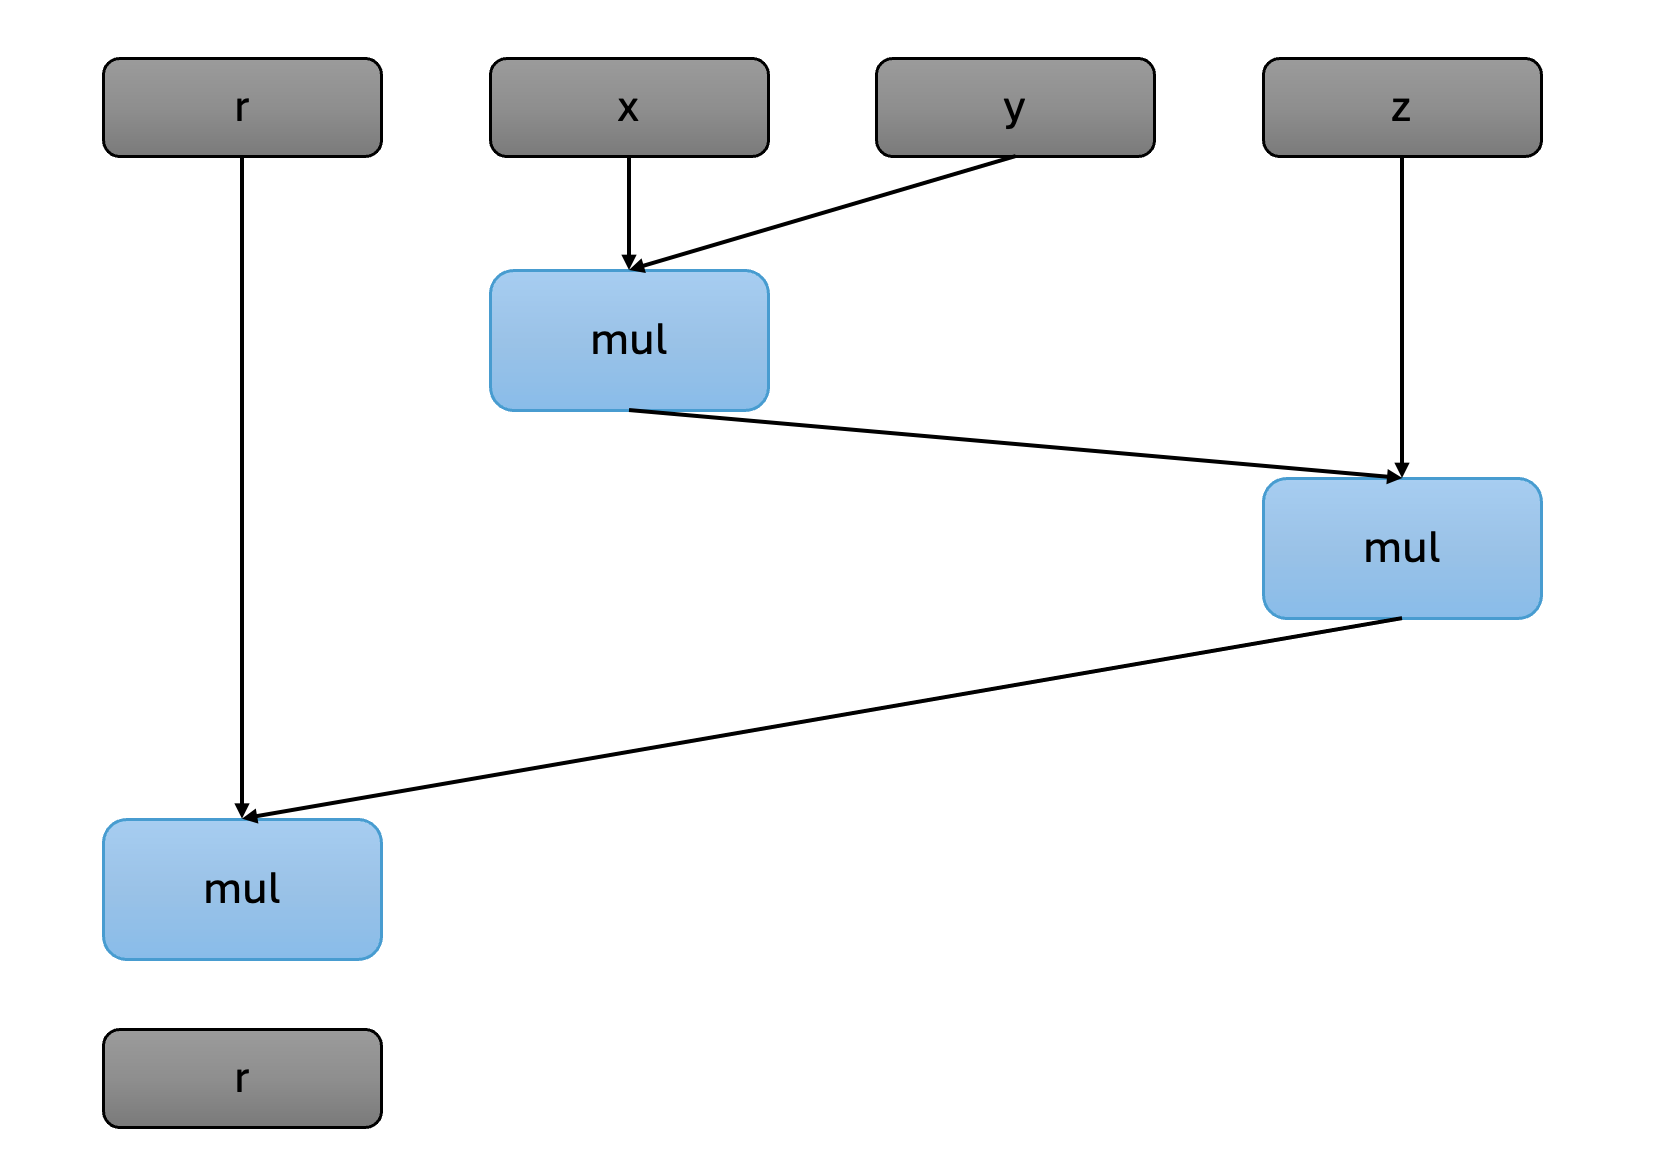
\includegraphics[width=0.5\textwidth]{fig3}
	\end{figure} \\
	The CPE is 1.67 clock cycles.
	\item For the equation $r = r*(x*(y*z))$. \\
	\begin{figure}[h]
		\centering
		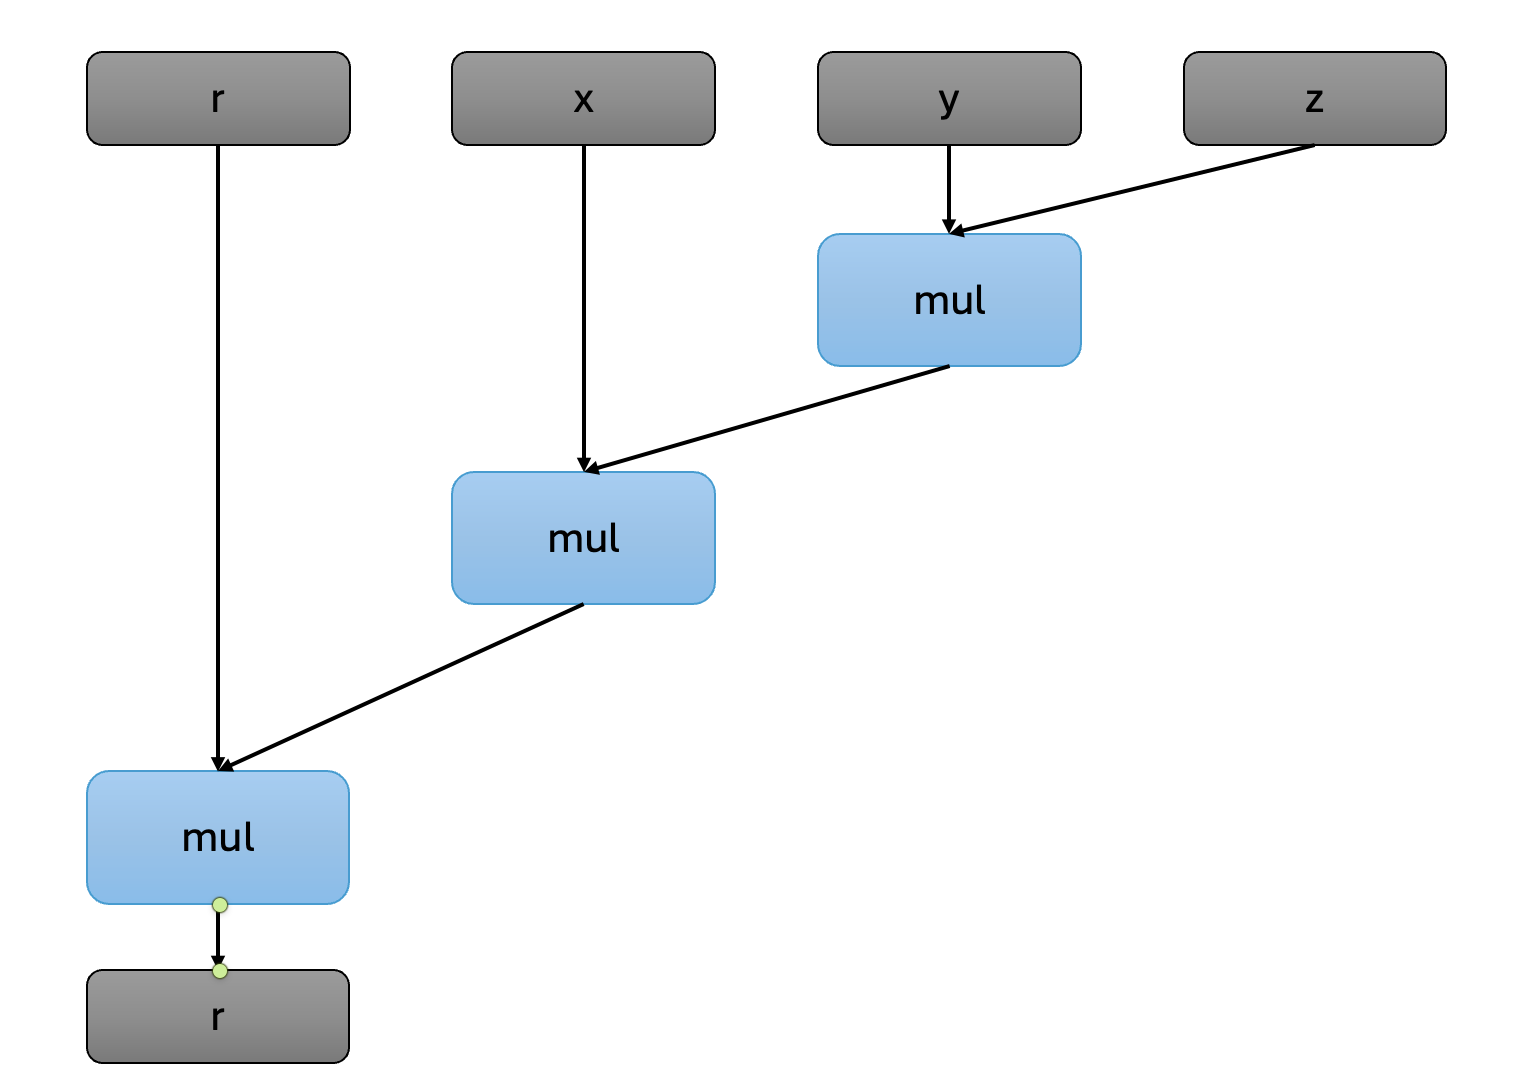
\includegraphics[width=0.5\textwidth]{fig4}
	\end{figure} \\
	The CPE is 1.67 clock cycles.
	\item For the equation $r = (r*x)*(y*z)$. \\
	\begin{figure}[h]
		\centering
		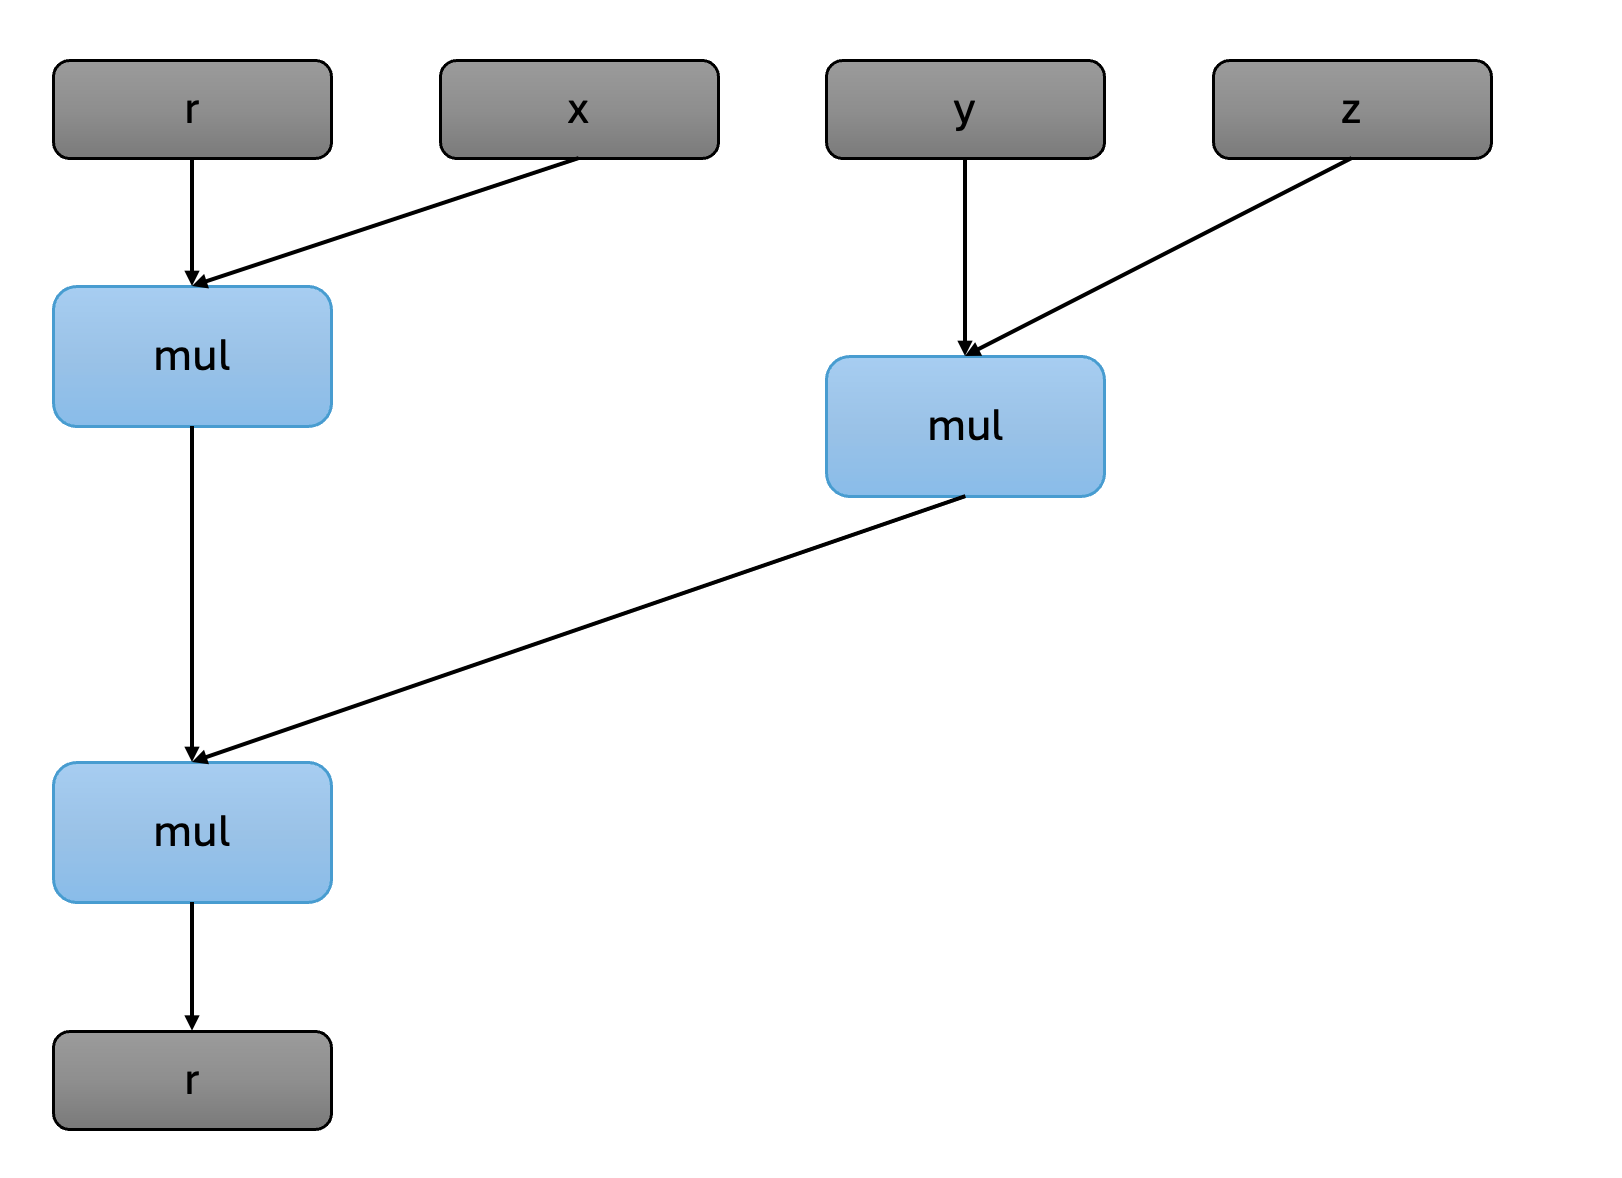
\includegraphics[width=0.5\textwidth]{fig5}
	\end{figure} \\
	The CPE is 3.33 clock cycles. 
\end{itemize}
\end{document}
